\documentclass[12pt, a4paper]{article}
\usepackage{graphicx} % Required for inserting images
\usepackage[top=1cm, bottom=2cm, left=1cm, right=1cm]{geometry}
\usepackage{parskip}

\graphicspath{{images/}}
\setlength{\parindent}{0cm}
\parskip 1.5ex


\title{Task 1 - SDLC Models}
\date{}
\begin{document}
\maketitle
\section{Waterfall Model}
The Waterfall Model is a linear and sequential approach to software development. It consists of distinct phases that must be completed in order, resembling a waterfall flowing downwards. The simple layout is easy to understand, with requirements properly defined for well-understood milestones. However, this model lacks the flexibility to accommodate changes once the development cycle has begun due to the rigid nature of requirements upfront.
The model includes the following stages:

\textbf{Requirements Analysis}: Gathering and documenting the requirements for the software system.

\textbf{Design}: Creating a high-level design and architecture based on the requirements.

\textbf{Implementation}: Writing code and developing the software based on the design.

\textbf{Testing}: Verifying and validating the software against the requirements and design.

\textbf{Deployment}: Installing and deploying the software in the production environment.

\textbf{Maintenance}: Providing ongoing support, updates, and software maintenance.

\begin{figure}[h]
    \centering
    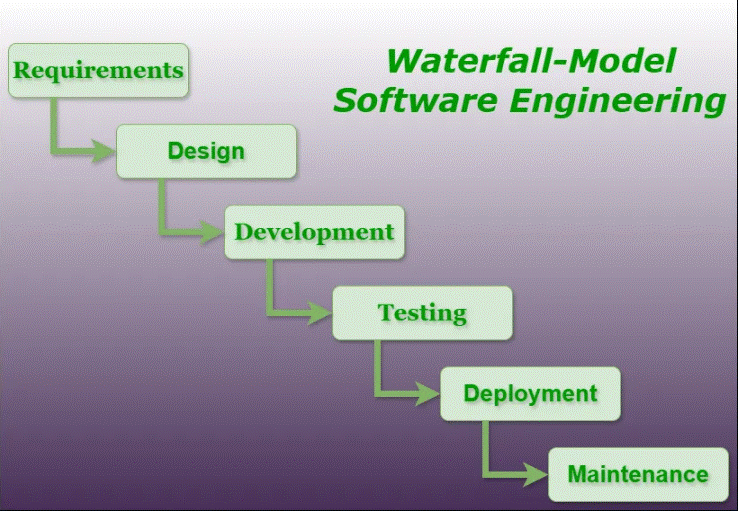
\includegraphics[width=0.5\textwidth]{images/waterfall-model.png}
    \caption{Waterfall Model (Source: GeeksforGeeks)}
    \label{fig:waterfall}
\end{figure}

\section{V-Shaped Model}
The V-Shaped model is similar to the Waterfall Model in its sequential development cycle but emphasises testing at each stage. The model follows a V-shaped pattern, where the left side represents the development phases, and the right side represents the corresponding testing phases. This ensures early detection of defects and reduces the cost of fixing issues further in the development lifecycle.

\begin{figure}[h]
    \centering
    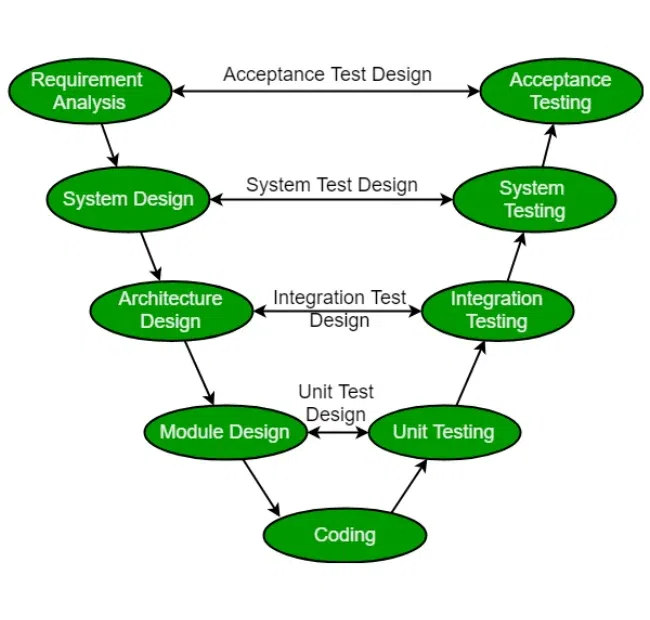
\includegraphics[width=0.5\textwidth]{images/v-model.png}
    \caption{V-Shaped Model (Source: GeeksforGeeks)}
    \label{fig:v-model}
\end{figure}

\section{Rapid Application Development Model}
The Rapid Application Development (RAD) model is a short development cycle prioritising rapid prototyping and iterative development. RAD involves building small prototypes quickly to gather useful feedback and make necessary adjustments. This model is for projects with evolving requirements or tight deadlines, as it emphasises rapid delivery of software increments.
The RAD model stages are:

\textbf{Requirements Planning}: Identifying and prioritising the key requirements for the software.

\textbf{User Design}: Involving end-users in the design process to rapidly prototype and iterate on user interfaces and functionality.

\textbf{Construction}: Rapidly building the software using iterative development cycles, focusing on delivering working prototypes quickly.

\textbf{Cutover}: Transitioning the software from development to production, including data migration and user training.

\textbf{Maintenance}: Providing ongoing support and maintenance for the software, incorporating feedback and making continuous improvements.


\begin{figure}[h]
    \centering
    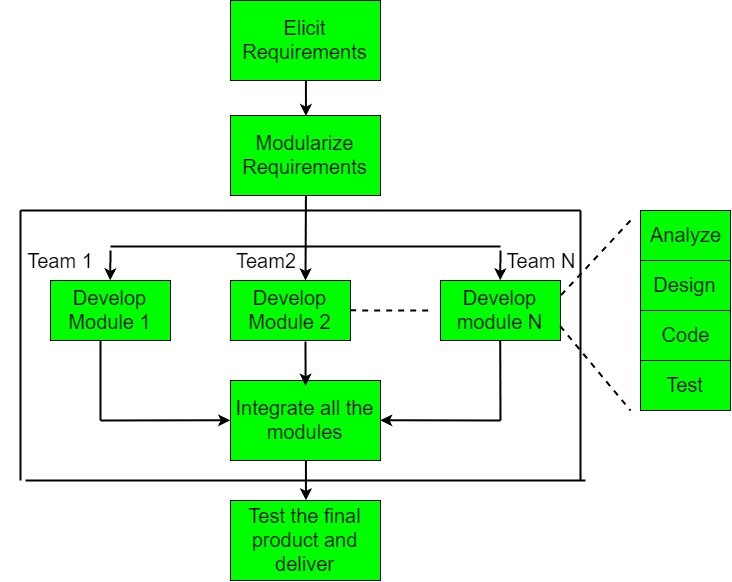
\includegraphics[width=0.5\textwidth]{images/RAD-model.jpg}
    \caption{RAD Model (Source: GeeksforGeeks)}
    \label{fig:RAD}
\end{figure}

\section{Spiral Model}
The Spiral Model combines the iterative prototyping approach with the waterfall model's systematic development. It consists of multiple cycles, each of which includes four phases: planning, risk analysis, engineering, and evaluation. The model begins with a small set of requirements and iteratively expands upon them in subsequent cycles. The model emphasises risk management and accommodates changes throughout the development process.
Spiral model includes the following stages:

\textbf{Planning}: Identifying objectives, constraints, and alternatives for the software project.

\textbf{Risk Analysis}: Evaluating potential risks and uncertainties associated with the project, including technical, schedule, and cost risks.

\textbf{Engineering}: Developing the software using iterative cycles, each of which includes requirements analysis, design, implementation, and testing.

\textbf{Evaluation}: Reviewing and assessing the project, including the identification of risks and potential changes to the project plan.

\begin{figure}[h]
    \centering
    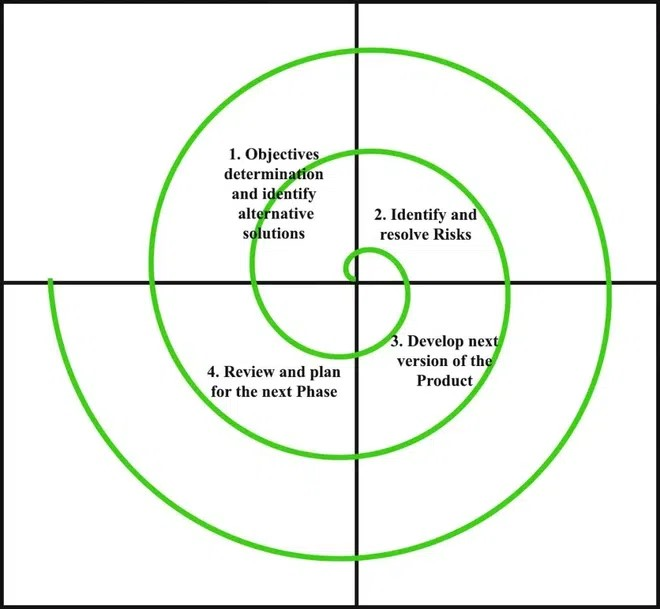
\includegraphics[width=0.5\textwidth]{images/spiral-model.jpg}
    \caption{Spiral Model (Source: GeeksforGeeks)}
    \label{fig:Spiral}
\end{figure}

\section{Agile Model}
The Agile Model is an iterative and incremental approach that emphasises adaptive planning, iterative delivery, and continuous improvement. Agile methods, such as Scrum and Kanban, prioritise collaboration, flexibility, and customer satisfaction. The development process is divided into short iterations called sprints, during which cross-functional teams deliver working software increments. Agile promotes rapid response to change and enables teams to deliver high-quality software efficiently.

\textbf{Requirement Gathering}: Identify requirements from the customer and plan time and work allocation to build the project. This allows for the evaluation of technical and economical feasibility.

\textbf{Design the Requirements}: Show new features and application to existing software through user-flow diagrams and UML diagrams. Wireframes and the design of the user interfaces are conducted at this stage.

\textbf{Construction / Iteration}: Start project work with aims to deploy a working product.

\textbf{Testing / Quality Assurance}: Testing such as unit testing, integration testing, and system testing is performed.

\textbf{Deployment}: Deploy the working project to end users.

\textbf{Feedback}: Gather feedback on product and correct bugs.


\begin{figure}[h]
    \centering
    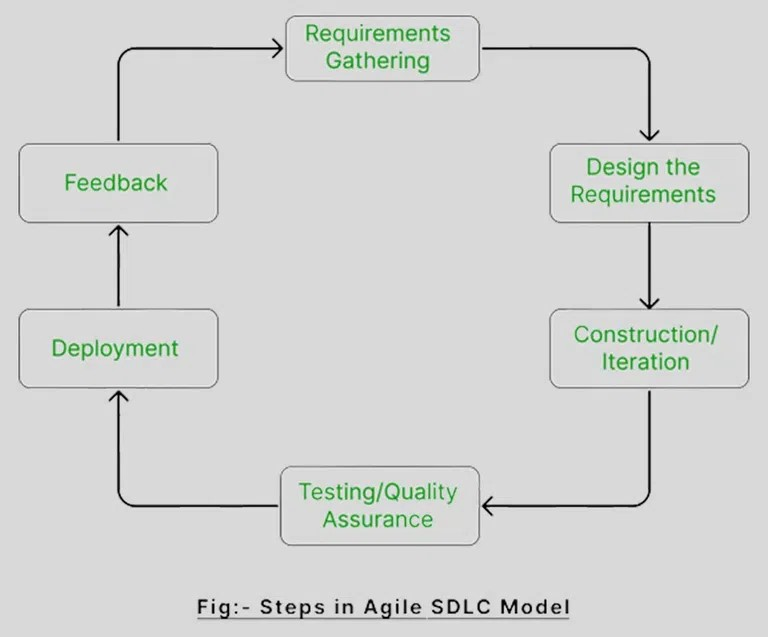
\includegraphics[width=0.5\textwidth]{images/agile-model.jpg}
    \caption{Steps in Agile Model (Source: GeeksforGeeks)}
    \label{fig:Agile}
\end{figure}

\end{document}
